\section{Methodology}
\label{sec:methodology}

This section discusses the characteristics and source of geographic map data,
various clustering techniques and algorithms to find the shortest
path between two data points.

\subsection{Geographic Dataset}
The data for this project will be collected from OpenStreetMap~\cite{osm},
which is an open source platform for maintaining map data of the entire earth.
There are several sources of getting the data, e.g., extracting directly from
the website for a small region or the entire planet, or continent, country or
state based data from Geofabrik Download Server~\cite{geo_dl_server}, etc.
Data normally comes in the human-readable XML formatted .osm files.
A basic format of the data presenting a datapoint by
$node$ and a connected path by $way$ XML DOM element.

The $node$ and $way$ information can be used to construct a weighted adjacency
matrix denoting the entire map, where weight of an edge is the distance between
two nodes.

%In the pre-processing stage, if the whole adjacency matrix is too large for
%the system memory, this can be written to a file and kept in storage devices.
%Later, according to the application performance requirements, density of the
%data can be reduced by only keeping the vertices that are the intersection
%points of three or more edges and update weight accordingly,
%because intersection of two edges actually will denote a single road.

\subsection{Clustering Techniques}
One of the most vital goals of this project is to perform research on different
clustering techniques when applied on different graph datasets. We have conducted a thorough study starting from very basic clustering like K-means
and hierarchical clustering to advanced techniques discussed in
Sec.~\ref{sec:literature_survey}.~\cite{structural_attribute_similarity_clustering, deep_representation_graph_clustering, parallel_graph_algorithm}
Specifically, some assumptions regarding transportation network can be leveraged
to set as constraints in the clustering techniques in order to simplify the transportation network graph processing and also to acquire faster convergence and ensure higher parallelism with the help of clustering. 
\subsubsection{Shortest Path Parallel Algorithm}
Using the above heuristics, the algorithm for finding a shortest
path between two vertices after clustering can be devised
as mentioned in Algorithm~1.

\begin{algorithm}[!htb]
    \label{alg:shortest_path_with_clustering}
    \caption{Find Shortest Path with Clustering}
    \begin{algorithmic}[1]
    \renewcommand{\algorithmicrequire}{\textbf{Input:}}
    \renewcommand{\algorithmicensure}{\textbf{Output:}}
    \REQUIRE graph, src, dest, cluster\_list
    \ENSURE  path

	\STATE Create subgraphs using clustering technique
	\STATE Construct $graph_c$ representing the gateway nodes as nodes and the weighted connection between them as edges. Both inter and intra cluster gateway connections are taken into consideration.
	\IF {($compute\_node == master$)}
		\IF {($src.cluster\_id == dest.cluster\_id$)}
			\STATE Send both src and dest information to $cluster\_list[src.cluster\_id]$
		\ELSE
			\STATE Send $src$ to $cluster\_list[src.cluster\_id]$
			\STATE Send $dest$ to $cluster\_list[dest.cluster\_id]$
			\STATE Apply $Find Shortest Path$ in $graph_c$
			\STATE Merge the $shortest\_paths$ after getting required information from slaves
			\RETURN $path$ found by the $shortest\_path$ search algorithm
		\ENDIF
	\ELSIF{($compute\_node == slave$)}
		\STATE $cluster = cluster\_list[compute\_node]$
		\IF {($src.cluster\_id == dest.cluster\_id$)}
    		\STATE $Find Shortest Path$ with $(cluster, src, dest)$
   		\ELSE
    		\IF {($src \in cluster$)}
    			\STATE Apply $Find Shortest Path$\\ with $(cluster, src, gateways)$
    		\ELSIF {($dest \in cluster$)}
    			\STATE Apply $Find Shortest Path$\\ with $(cluster, gateways, dest)$
    		\ELSE
    			\STATE Apply $Find Shortest Path$\\ with $(cluster, gateways, gateways)$
    		\ENDIF
   		\ENDIF
    	\STATE Send required information to master
    \ENDIF
    \end{algorithmic}
\end{algorithm}

\subsection{Algorithm Description}
Our proposed algorithm can be divided into 4 steps.
\begin{itemize}
    \item{Clustering graph}
    \item{Gateway Detection}
    \item{Intra-cluster shortest path detection}
    \item{Inter-cluster shortest path detection}
\end{itemize}
\subsubsection{Clustering Graph} As the transport network will not change rapidly over time, we are doing the clustering in a pre-processing step. This pre-processing phase will not affect the run time of our proposed algorithm. In this phase, we are extracting the data from the web and feeding the necessary information to our data structure. Then we are passing the data through various clustering algorithms e.g. Kmeans clustering, Agglomerative clustering. For our proposed algorithm, we are clustering entire dataset into small segments.
\begin{figure}[h]
\centering
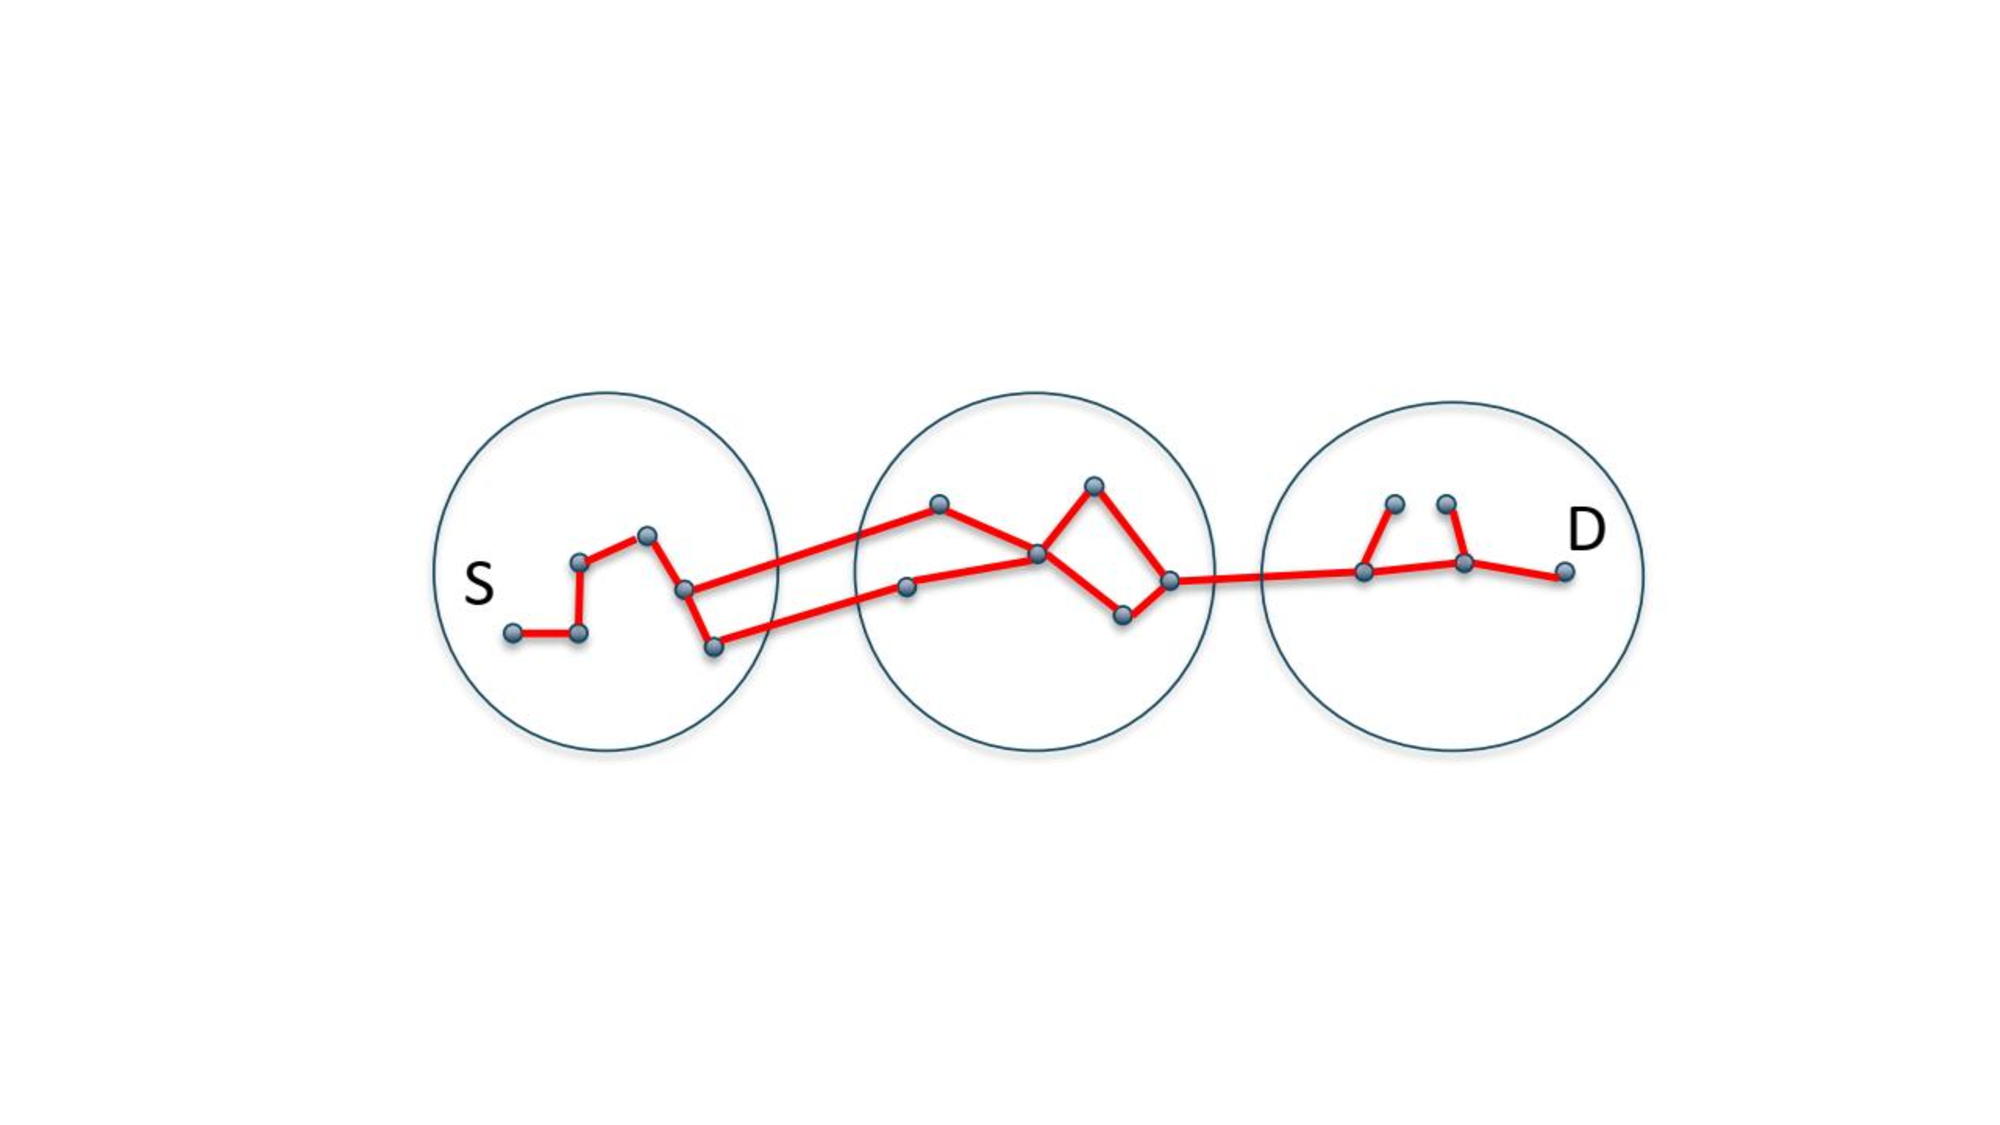
\includegraphics[width=0.4\textwidth]{images/Clustering_graph.pdf}
\caption{Graph clustering}
\label{fig:graph_clustering}
\end{figure}
In \figurename~\ref{fig:graph_clustering}, the whole graph has been partitioned into the 3 small clusters making it suitable for running our proposed distributed algorithm.
\subsubsection{Gateway Detection} After clustering the dataset, there are still some gateway edges, which connect the clusters. These gateway edges are necessary for computing the overall shortest path. For detecting these edges, we select the nodes who have at least one of their edges connected to any of  the nodes in other cluster. We call this nodes gateway nodes. In this step, alongside with detecting gateway edges we also detect the subgraphs of inter-cluster gateways.

\begin{figure}[!htb]
\centering
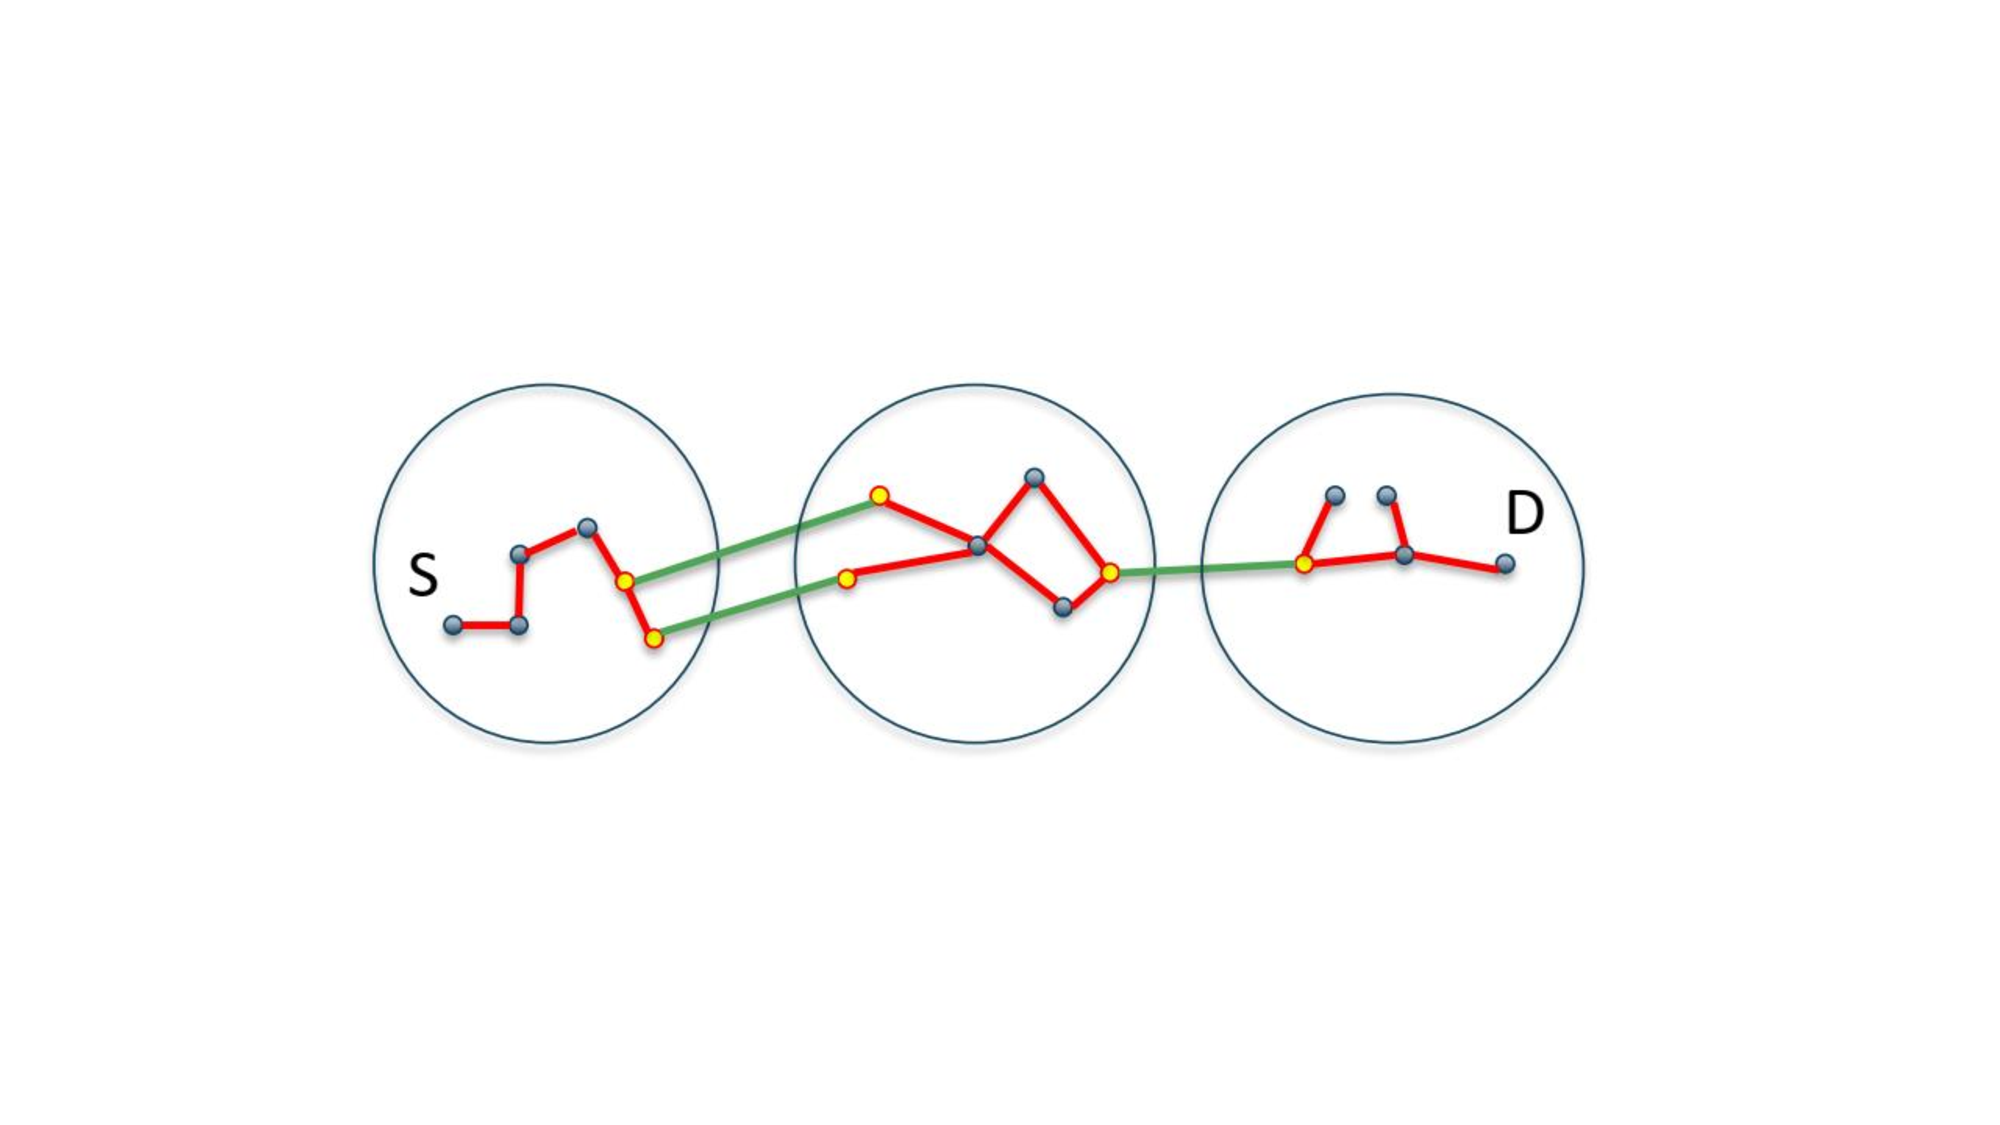
\includegraphics[width=0.4\textwidth]{images/Gateway_detection.pdf}
\caption{Detection of gateways}
\label{fig:gateway_detection}
\end{figure}
In \figurename~\ref{fig:gateway_detection}, the gateway nodes have been marked with yellow and the gateway edges have been colored green. These gateway edges connects the three clusters externally.

\subsubsection{Intra-cluster shortest path detection} For detecting the shortest path in the clusters we run single source shortest path algorithms e.g. dijkstra's algorithm, individually in the different clusters. Based on the given source and destination we classify the clusters as source cluster, destination cluster and intermediate clusters. In the source cluster, we find all the shortest paths from source to gateway nodes. In case of intermediate clusters, we determine the shortest paths between all possible gateways. In the destination cluster, shortest path is detected from all gateway points to the destination nodes. \\
\begin{figure}[!htb]
\centering
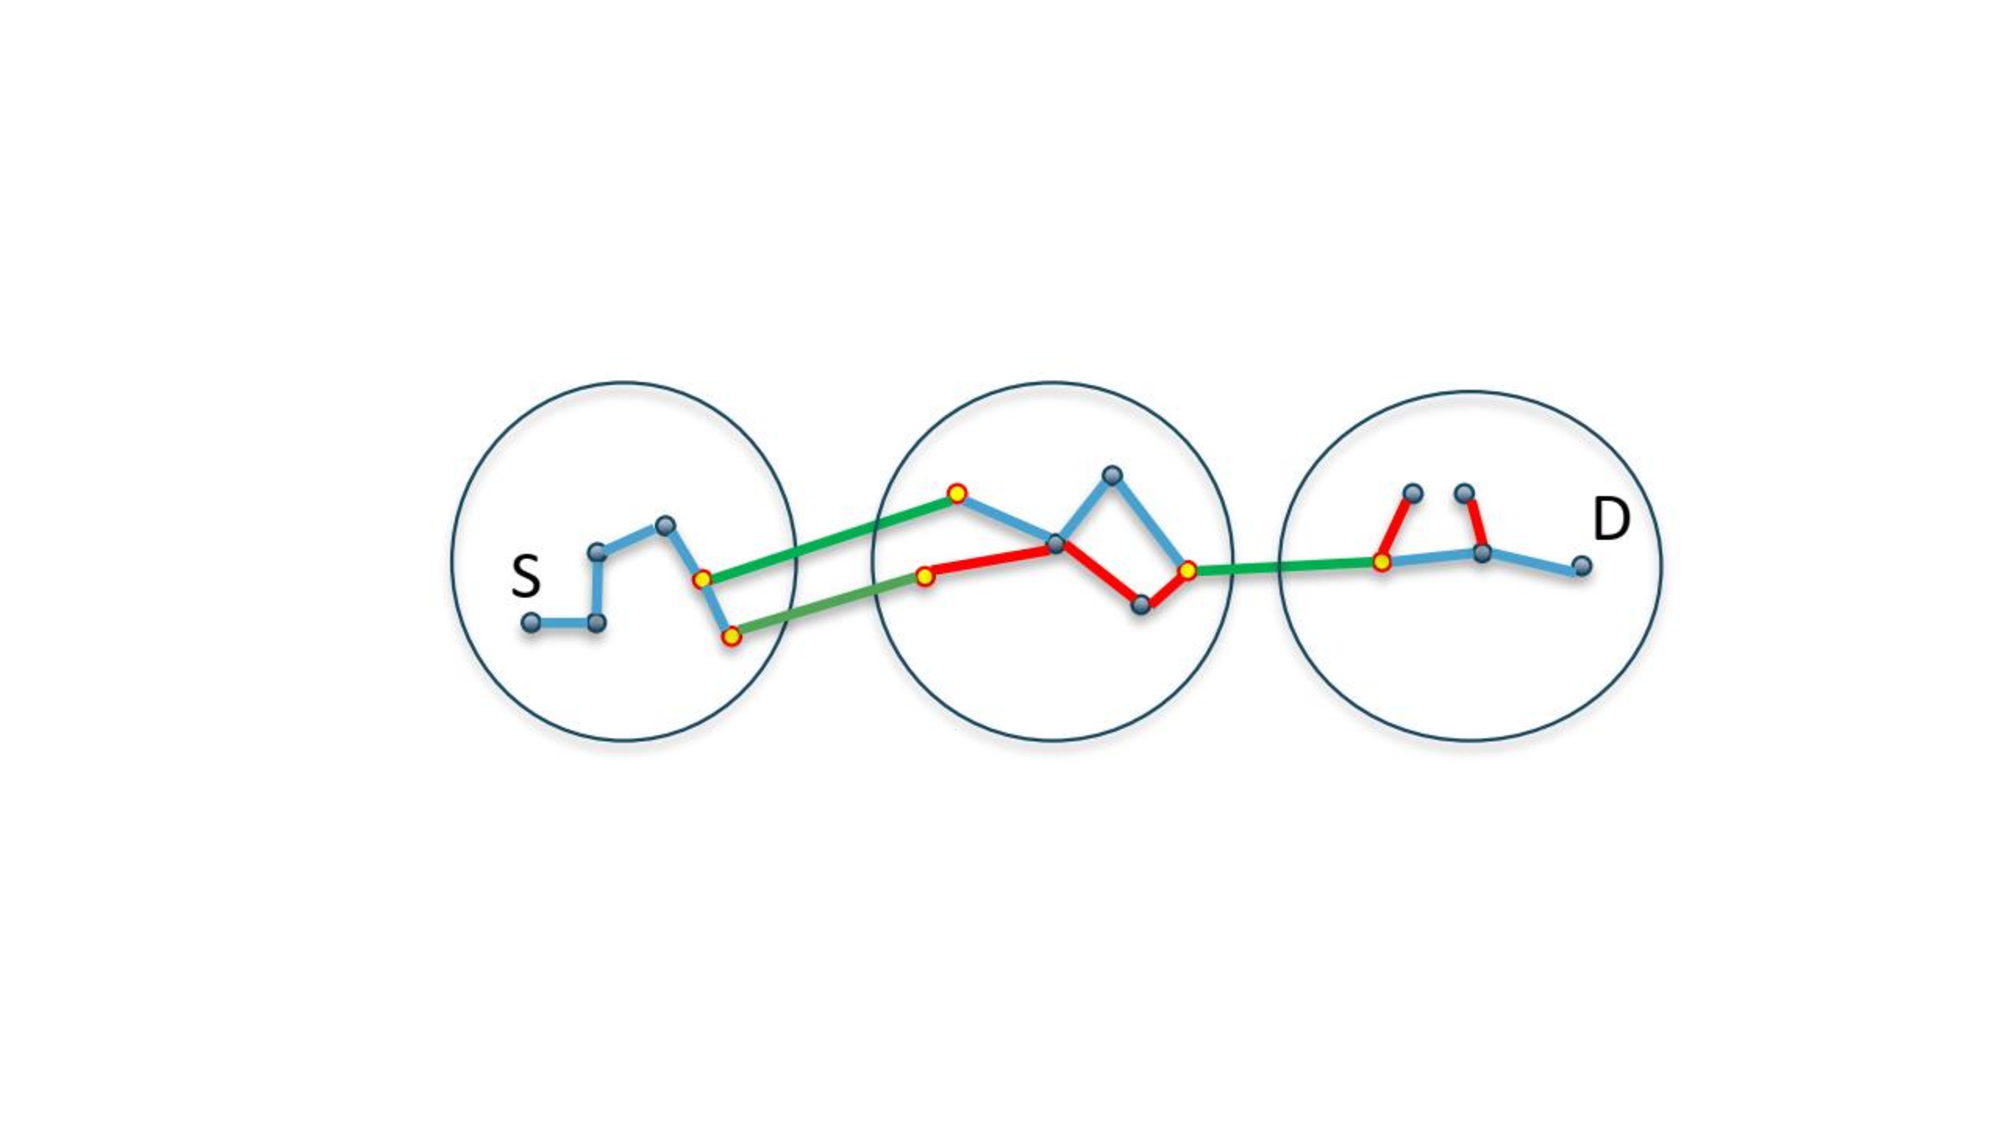
\includegraphics[width=0.4\textwidth]{images/Intra_cluster_sssp.pdf}
\caption{Detection of intra-cluster shortest paths}
\label{fig:intra_clus_sp}
\end{figure}
In \figurename~\ref{fig:intra_clus_sp}, in the source cluster, marked as S, we compute the shortest path from source node to the two gateway nodes colored yellow. In the intermediate cluster, shortest paths are detected between all possible gateways. in the destination cluster, marked as D, we compute the shortest paths from gateway nodes to destination node.
\subsubsection{Inter-cluster shortest path detection} In this step, shortest paths calculated between inter-cluster edges. After creating the subgraphs of gateway nodes and edges, single source shortest path algorithm is applied on each gateway subgraph. the goal is to find the shortest inter-cluster paths.

\begin{figure}[!htb]
\centering
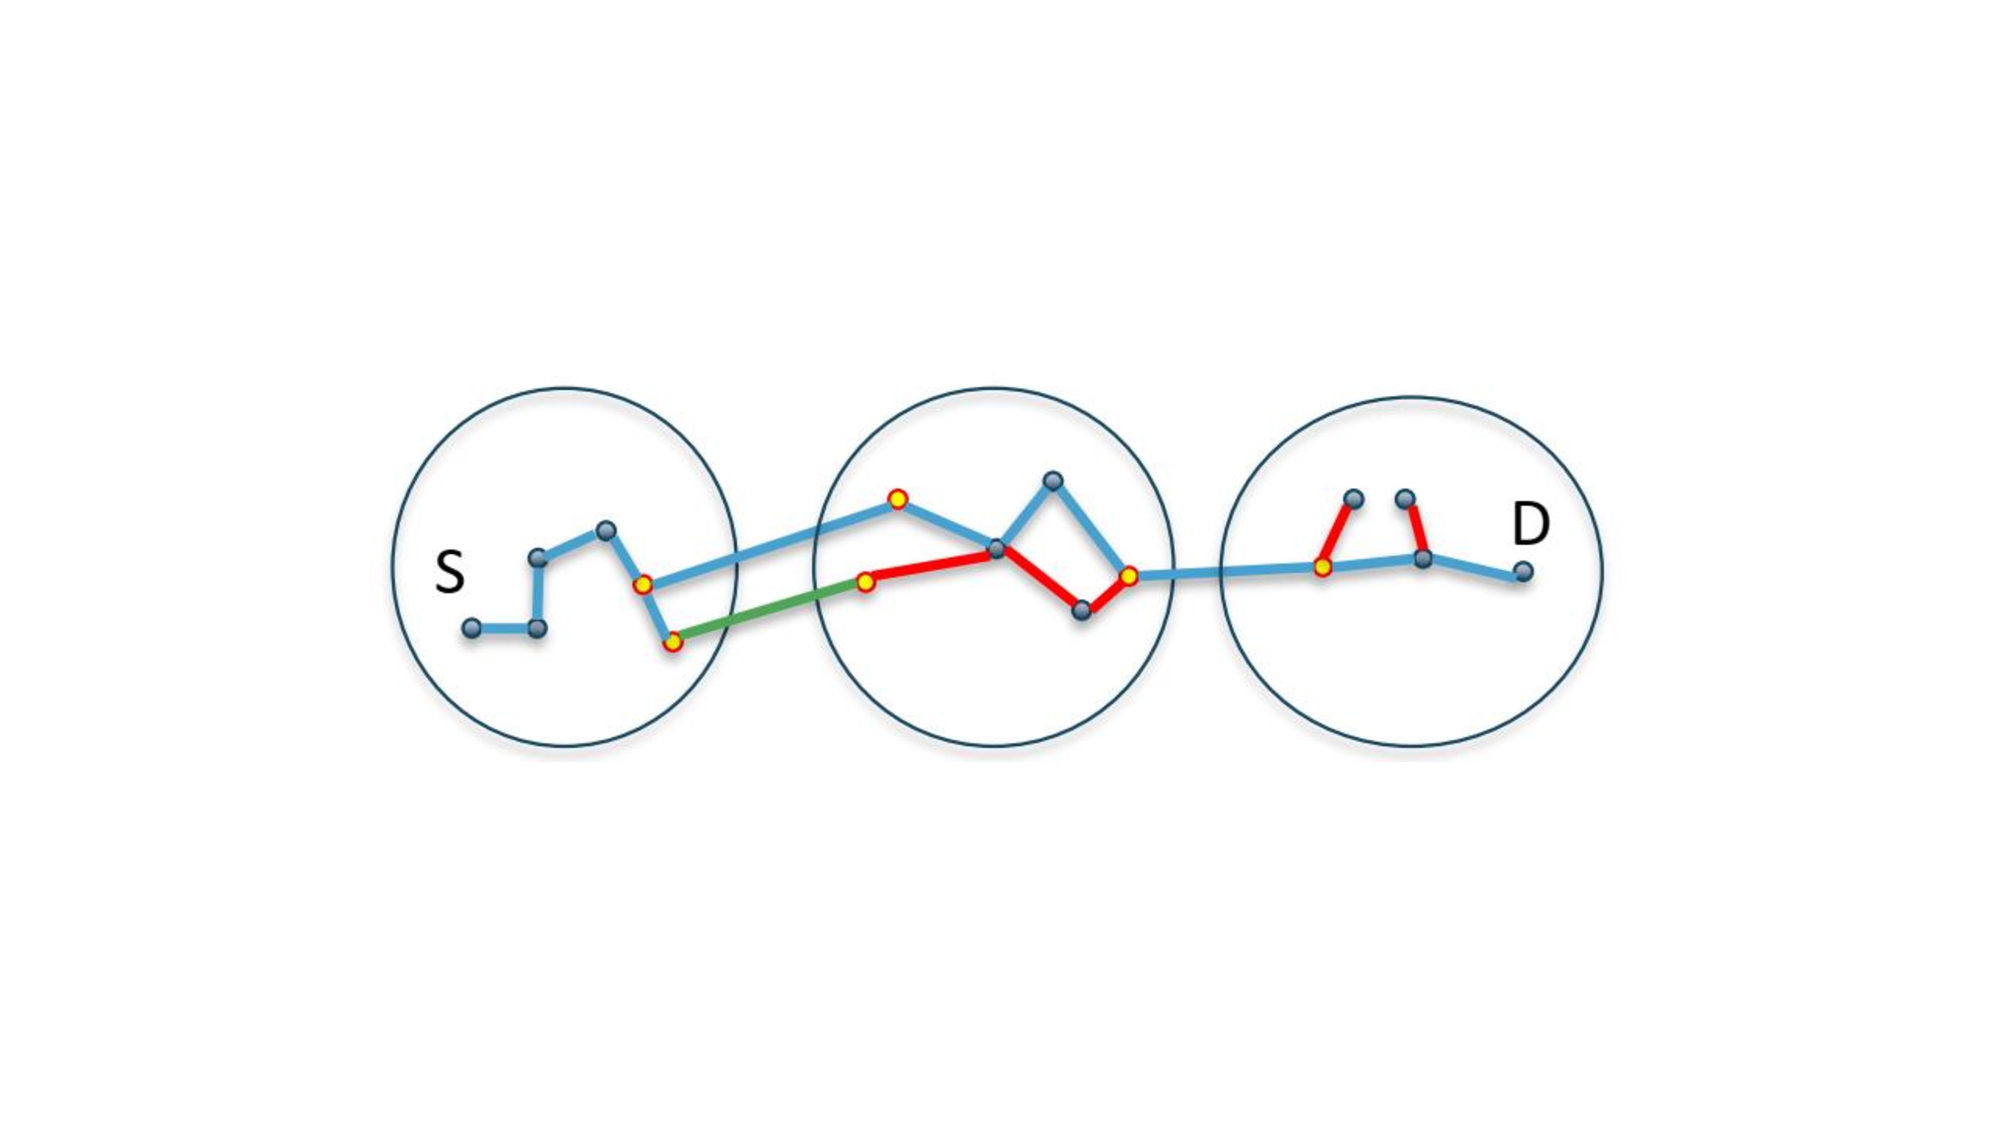
\includegraphics[width=0.4\textwidth]{images/Inter_cluster_sssp.pdf}
\caption{Detection of inter-cluster shortest paths}
\label{fig:inter_cluster_sp}
\end{figure}
In \figurename~\ref{fig:inter_cluster_sp}, the inter-cluster shortest paths have been colored as blue.